% =============================================================================
% ReBel — §5 Experiments
% NeurIPS 2026
% (Section heading and \label{sec:experiments} are in main.tex)
% =============================================================================

We assess ReBel in two demanding multi-step interactive domains:
ALFWorld~\citep{shridhar2021alfworld}, a benchmark for household tasks in text
environments, and WebShop~\citep{yao2022webshop}, which evaluates navigation and
decision-making in a simulated e-commerce setting.
The experimental analysis is structured around four central questions:
\textbf{(Q1)}~Does ReBel surpass both episode-level and existing step-level
baselines?
\textbf{(Q2)}~What is the marginal impact of each architectural component?
\textbf{(Q3)}~How effectively does HiBO mitigate the singleton group problem?
\textbf{(Q4)}~Can adaptive differential decay address reward shaping bias?


% -----------------------------------------------------------------------------
\subsection{Experimental Setup}
\label{sec:exp_setup}

\paragraph{Environments.}
\textbf{ALFWorld}~\citep{shridhar2021alfworld} features six household task types
(pick-and-place, pick-two, pick-heat, pick-cool, pick-clean, look-at-object),
with episode lengths ranging from 8 to 30 steps.
Each training batch contains 16 prompts; evaluation uses the full 128-task
validation set at generalization level~0 (rooms seen during training).
\textbf{WebShop}~\citep{yao2022webshop} requires the agent to fulfill natural
language purchase requests by navigating a simulated e-commerce website via
\texttt{search[...]} and \texttt{click[...]} actions.
Episodes are capped at 15 steps, and rewards are continuous ($r \in [0,1]$),
reflecting how well the purchased product matches the attribute, option, and
price constraints of the instruction.

\paragraph{Base model and SFT cold-start.}
All methods initialize from an identical supervised fine-tuning (SFT) checkpoint.
We fine-tune Qwen2.5-1.5B-Instruct~\citep{qwen2.5} on 390 hindsight-annotated
expert trajectories (ALFWorld) or 500 trajectories (WebShop) for 90 epochs.
As a control, applying RL directly from the raw pretrained model (no SFT) yields
only 7.8\% success rate after 100 RL epochs---confirming that the cold-start SFT
phase is indispensable.
Concretely, the model must learn to emit well-formed \texttt{<belief>} JSON
\emph{before} the grouping-based advantage signal can carry any useful information;
without this structural prerequisite, exploration under RL degenerates.

\paragraph{Baselines.}
Four methods are compared within a unified training protocol:
\begin{itemize}[leftmargin=1.5em,itemsep=2pt]
  \item \textbf{GRPO}~\citep{shao2024deepseekmath}: Episode-level advantage via
    group relative normalization.
    Prompt format: \texttt{<think>...<action>}.
  \item \textbf{GiGPO}~\citep{feng2025gigpo}: Step-level advantage via exact
    observation hash grouping, combined with episode-level GRPO.
    Same \texttt{<think>} prompt format.
  \item \textbf{GiGPO + Belief}: GiGPO with the structured belief
    prompt \texttt{<belief>\{JSON\}</belief><action>}; configuration
    matched to V10-C1 (same hyperparameters, different prompt only).
  \item \textbf{ReBel (ours)}: HiBO grouping with adaptive differential belief
    reward curriculum.
    Prompt: \texttt{<belief>\{JSON\}</belief><reasoning>...<action>}.
\end{itemize}

\paragraph{Hyperparameters.}
All methods share identical optimization settings: learning rate $10^{-6}$ (Adam),
one PPO epoch per rollout batch, KL regularization coefficient 0.001
(low-variance estimator), 16 rollout trajectories per prompt, and 100 training
epochs.
Beyond these shared settings, ReBel applies asymmetric clipping
($\epsilon_{\text{low}}=0.2$, $\epsilon_{\text{high}}=0.28$), clip-covariance
entropy protection (range $[0.0, 0.3]$), and an invalid action penalty
($\lambda=0.1$).
Training runs on 8$\times$A100 GPUs (ALFWorld) and 4$\times$A100 GPUs (WebShop).
Full configuration details appear in Appendix~\ref{app:config}.

\paragraph{Metrics.}
\textbf{Peak SR}: the highest validation success rate observed across all epochs.
\textbf{Final SR}: success rate at epoch~100.
\textbf{Late-Avg SR}: mean success rate over the last five evaluation checkpoints
(epochs 80--100), which reflects sustained stability rather than an isolated peak.
For WebShop, a trajectory is considered successful when its task score is
$\geq 0.5$.


% -----------------------------------------------------------------------------
\subsection{Main Results}
\label{sec:main_results}

% --- Table 1 ---
\begin{table}[t]
  \centering
  \caption{%
    \textbf{Main results on ALFWorld} (seed\,=\,42, 128-task validation set).
    $\Delta_{\text{GRPO}}$ is the absolute improvement in peak SR over the
    GRPO baseline.
    GiGPO + Belief borrows the V10-C1 configuration (same hyperparameters;
    see text).
  }
  \label{tab:main_results}
  \vspace{4pt}
  \small
  \renewcommand{\arraystretch}{1.15}
  \begin{tabular}{@{}lcccc@{}}
    \toprule
    \textbf{Method}
      & \textbf{Peak SR (\%)}
      & \textbf{Final SR (\%)}
      & \textbf{Late-Avg SR (\%)}
      & $\boldsymbol{\Delta}_{\textbf{GRPO}}$ \\
    \midrule
    GRPO
      & 82.0 & 82.0 & 78.7 & --- \\
    GiGPO (\texttt{<think>})
      & 91.4 & 82.0 & 86.7 & $+$9.4 \\
    GiGPO (\texttt{<belief>})
      & 94.5 & 86.7 & 90.0 & $+$12.5 \\
    \textbf{ReBel (ours)}
      & \textbf{95.3} & \textbf{89.1} & \textbf{91.1} & $\mathbf{+13.3}$ \\
    \bottomrule
  \end{tabular}
\end{table}

Table~\ref{tab:main_results} presents the comparison on ALFWorld.
Three observations stand out.

\textit{First}, step-level credit assignment is the single largest contributor.
Replacing episode-level GRPO with GiGPO raises peak SR by 9.4 percentage points
(82.0\% $\to$ 91.4\%).
In multi-step tasks where a single misstep can cascade into a failed trajectory,
fine-grained temporal credit carries far more information than the episodic
return alone.

\textit{Second}, structured belief representation amplifies the step-level signal.
Switching from GiGPO's \texttt{<think>} format to \texttt{<belief>} JSON---while
holding the grouping mechanism constant (still exact observation hash)---lifts
peak SR by a further 3.1\,pp (91.4\%\,$\to$\,94.5\%, Table~\ref{tab:main_results}).
This gain is attributable to the richer grouping information available in
belief-format trajectories, not to any algorithmic change in the grouping or
reward mechanism.
For comparison, adding belief prompting \emph{without} a step-level mechanism
(B1 in Table~\ref{tab:ablation}) yields only a marginal and unstable improvement
($+$1.6\,pp peak, $-$2.0\,pp late-average), confirming that the representation
benefit is contingent on having a credit-assignment mechanism to exploit it.

\textit{Third}, the full ReBel system (HiBO $+$ adaptive curriculum) adds a
further $+$0.8\,pp over the GiGPO\,$+$\,Belief baseline (94.5\%\,$\to$\,95.3\%).
The 0.8\,pp peak difference is modest in isolation; its interpretation requires
the targeted ablation in Table~\ref{tab:ablation_v11}, which decomposes this
jointly attributed step into the curriculum's and HiBO's individual contributions.
The Late-Avg SR comparison (91.1\% vs.\ 90.0\%) is consistent with the full
system providing more stable learning at the performance frontier.

% --- Figure: Training curves ---
\begin{figure}[t]
  \centering
  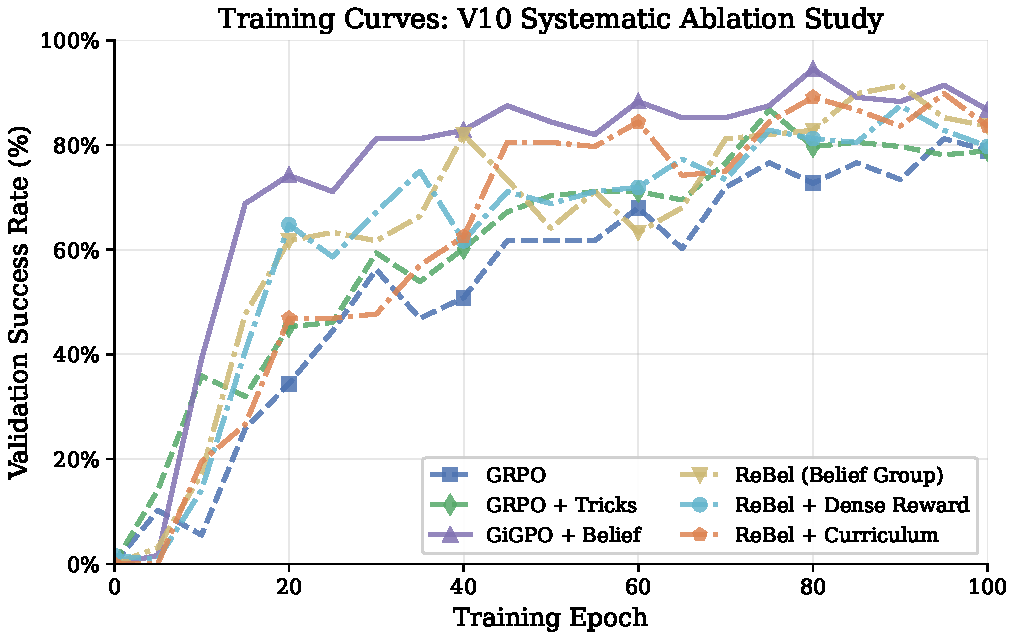
\includegraphics[width=\linewidth]{../code/rebel_test_results/v11_final/paper_figures/fig1_training_curves_v10.pdf}
  \caption{%
    \textbf{Validation success rate over 100 training epochs} (ALFWorld, V10 systematic ablation).
    GiGPO-based methods (C1, C2, D1, E1) reach 80\% SR by epoch~30, while episode-level
    methods (A1, A2, B1) take 3--5$\times$ longer.
    GRPO + Belief (B1) exhibits the largest late-stage variance, confirming that
    belief prompting without step-level mechanisms is destabilising.
  }
  \label{fig:training_curves}
\end{figure}

\paragraph{Training dynamics.}
Figure~\ref{fig:training_curves} traces validation SR across training.
GiGPO crosses 80\% by epoch~30; GRPO does not reach the same threshold until
epoch~95---a $>$3$\times$ acceleration.
The GRPO + Belief variant (B1) exhibits the highest late-stage variance
(8.2\% standard deviation over epochs 80--100, vs.\ 3.0\% for GiGPO + Belief),
a pattern that recurs throughout our ablations and underscores that structured
belief output is beneficial only when paired with a step-level mechanism able
to exploit its temporal structure.

% --- Table: Factor decomposition ---
\begin{table}[t]
  \centering
  \caption{%
    \textbf{Cumulative factor decomposition from GRPO to ReBel} (ALFWorld).
    Each row adds one component on top of the previous configuration.
    Marginal contributions are measured in peak SR.
  }
  \label{tab:factor_decomposition}
  \vspace{4pt}
  \small
  \renewcommand{\arraystretch}{1.15}
  \begin{tabular}{@{}lcc@{}}
    \toprule
    \textbf{Configuration} & \textbf{Cumulative Peak SR (\%)} & \textbf{Marginal $\Delta$} \\
    \midrule
    GRPO baseline                        & 82.0          & ---    \\
    $+$ Step-level advantage (GiGPO)     & 91.4          & $+$9.4 \\
    $+$ Structured belief prompting      & 94.5          & $+$3.1 \\
    $+$ HiBO $+$ Adaptive curriculum     & \textbf{95.3} & $+$0.8 \\
    \bottomrule
  \end{tabular}
\end{table}

\paragraph{Factor decomposition.}
Table~\ref{tab:factor_decomposition} traces the cumulative build-up from GRPO to
ReBel as individual components are added sequentially.
Step-level advantage delivers the bulk of the gain ($+$9.4\,pp);
structured belief format contributes $+$3.1\,pp by enriching the grouping signal
available to the step-level mechanism;
HiBO with adaptive curriculum adds the final $+$0.8\,pp at the performance
frontier, a regime where further gains are harder to obtain.

\textbf{Note on attribution.}
The $+$3.1\,pp attributed to belief format here (Table~\ref{tab:main_results},
GiGPO/think $\to$ GiGPO+Belief) reflects a \emph{representation change}:
identical GiGPO algorithm, different output format.
It is \emph{distinct} from the $-$3.1\,pp observed when the belief \emph{reward}
is removed from the full ReBel system (Table~\ref{tab:ablation_v11}, A3).
The numeric coincidence could mislead: in one context the $+$3.1 is the marginal
value of structured intermediate representation under step-level grouping;
in the other it is the marginal value of intrinsic reward under full ReBel.
The targeted ablation (Table~\ref{tab:ablation_v11}) should be consulted for
component-specific attribution within the ReBel system.


% -----------------------------------------------------------------------------
\subsection{Ablation Study}
\label{sec:ablation}

\paragraph{Systematic ablation (V10).}
We first conduct a seven-configuration controlled study that progressively introduces
components, enabling clean isolation of each factor's marginal effect.

% --- Table: V10 systematic ablation ---
\begin{table}[t]
  \centering
  \caption{%
    \textbf{Systematic component ablation} (ALFWorld, V10, seed\,=\,42).
    Seven configurations are added sequentially.
    The step-level advantage transition (C1\,vs.\,B1) is the dominant isolated gain.
    ``Isolated $\Delta$'' is the pairwise difference between adjacent rows.
  }
  \label{tab:ablation}
  \vspace{4pt}
  \small
  \renewcommand{\arraystretch}{1.15}
  \begin{tabular}{@{}clcccc@{}}
    \toprule
    & \textbf{Configuration}
      & \textbf{Peak SR (\%)} & \textbf{Late-Avg SR (\%)}
      & \multicolumn{2}{c}{\textbf{Isolated $\Delta$}} \\
    \cmidrule(lr){5-6}
    & & & & \textbf{Peak} & \textbf{Late-Avg} \\
    \midrule
    A1 & GRPO baseline                    & 81.2 & 78.7 & ---         & ---         \\
    A2 & \quad$+$ Training tricks         & 86.7 & 79.4 & $+$5.5      & $+$0.7      \\
    B1 & \quad$+$ Belief prompting        & 88.3 & 77.4 & $+$1.6      & $-$2.0      \\
    C1 & \quad$+$ Step-level adv.\ (obs)  & \textbf{94.5} & \textbf{90.0} & $\mathbf{+6.2}$ & $\mathbf{+12.6}$ \\
    C2 & \quad Belief hash grouping       & 91.4 & 86.6 & $-$3.1      & $-$3.4      \\
    D1 & \quad$+$ Dense belief reward     & 87.5 & 84.3 & $-$3.9      & $-$2.3      \\
    E1 & \quad$+$ Cosine decay            & 89.8 & 86.6 & $+$2.3      & $+$2.3      \\
    \bottomrule
  \end{tabular}
\end{table}

The ablation reveals four principal findings.

\textit{Step-level advantage is the most impactful component} (C1 vs.\ B1: $+$6.2\% peak,
$+$12.6\% late-average).
The late-average gap in particular---12.6 pp---reflects the cumulative benefit of
a high-quality credit signal over the full training run.

\textit{Observation-only grouping outperforms belief-only grouping} (C2 vs.\ C1: $-$3.1\%
peak).
When belief hash grouping replaces observation hashing, performance drops.
The causes are threefold: belief hashes are endogenous (they change as the policy
updates, yielding non-stationary grouping targets), early-training beliefs are noisy,
and the finer granularity of belief features reintroduces singleton groups.
This negative result directly motivated HiBO's hierarchical design: use observation
hashing as the primary layer, and fall back to belief abstraction only for singletons.

\textit{Dense intrinsic reward is harmful without curriculum} (D1 vs.\ C2: $-$3.9\%
peak).
From a reward shaping perspective~\citep{ng1999policy}, belief rewards are not
potential-based (they depend on model outputs, not purely on states), so they bias
the optimal policy: $\pi^*_{R + \alpha R_{\text{belief}}} \neq \pi^*_R$.
Cosine decay (E1) partially recovers this loss (+2.3\%), but the net effect is still
negative relative to C2 ($-$1.6\%).
Adaptive differential decay in ReBel resolves this by removing misaligned components
faster than well-aligned ones (see~\S\ref{sec:decay_analysis}).

\textit{Belief prompting is a necessary but insufficient condition} (B1 vs.\ A2).
B1 achieves 88.3\% peak but suffers the worst late-stage variance (8.2\% std
over epochs 80--100).
The same belief format with step-level grouping (C1) yields 94.5\% peak at 3.0\%
std---the information scaffold becomes useful only once a mechanism exists to exploit
its temporal structure.

% --- Figure: Factor contribution ---
\begin{figure}[t]
  \centering
  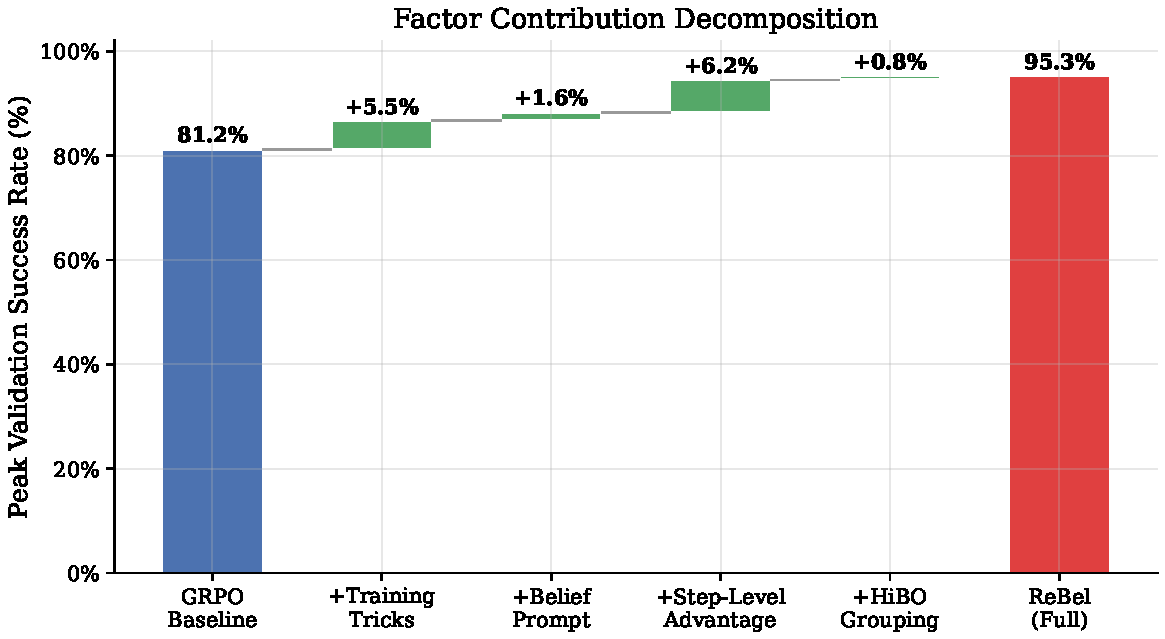
\includegraphics[width=0.85\linewidth]{../code/rebel_test_results/v11_final/paper_figures/fig4_factor_contribution.pdf}
  \caption{%
    \textbf{Factor contribution waterfall} (ALFWorld, V10).
    Green bars indicate positive marginal contributions; red bars indicate negative
    effects that motivated subsequent design revisions.
  }
  \label{fig:factor_waterfall}
\end{figure}

\paragraph{Targeted ablation (V11).}
To measure the specific contributions of HiBO, the belief reward, and adaptive
decay within the full ReBel system, we run three single-factor removal experiments
in the V11 setting.
Results are in Table~\ref{tab:ablation_v11}.

% --- Table: V11 targeted ablation ---
\begin{table}[t]
  \centering
  \caption{%
    \textbf{Targeted component ablation within ReBel} (ALFWorld, V11, seed\,=\,42).
    Each row removes one component from the full system.
    A4 (w/o adaptive decay) ran for 90 epochs before abnormal termination;
    peak SR is computed over the available epochs.
  }
  \label{tab:ablation_v11}
  \vspace{4pt}
  \small
  \renewcommand{\arraystretch}{1.15}
  \begin{tabular}{@{}lccc@{}}
    \toprule
    \textbf{Configuration}
      & \textbf{Peak SR (\%)}
      & \textbf{Final SR (\%)}
      & \textbf{Late-Avg SR (\%)} \\
    \midrule
    \textbf{ReBel Full (M5)}         & \textbf{95.3} & 89.1          & 91.1          \\
    A1: w/o HiBO (obs-only grouping) & 94.5          & 91.4          & 90.8          \\
    A3: w/o Belief Reward            & 92.2          & 91.4          & 88.6          \\
    A4: w/o Adaptive Decay           & 92.2          & \textbf{92.2} & \textbf{89.8} \\
    \bottomrule
  \end{tabular}
\end{table}

The comparison between ReBel Full and A1 (w/o HiBO) reveals an important nuance.
The peak SR gap is only $+$0.8\,pp, and A1's final SR (91.4\%) exceeds
ReBel Full's (89.1\%).
We interpret this inversion as follows: HiBO's denser advantage signal (covering
$\sim$76\% vs.\ $\sim$20\% of steps) enables the policy to explore and improve
more aggressively during training, resulting in a higher \emph{peak} but also
greater variance between the peak checkpoint and the endpoint.
In other words, HiBO's benefit is manifested as a wider peak-to-final spread,
not as a uniformly higher performance profile.
We acknowledge that this interpretation cannot be fully confirmed with
single-seed experiments; the key open question is whether the $+$0.8\,pp peak
advantage and HiBO's variance-reduction hypothesis would hold or amplify
across multiple seeds.

Removing the belief reward (A3) drops peak SR by 3.1\,pp (95.3\%\,$\to$\,92.2\%),
confirming that the intrinsic signal retains substantial value even as its
curriculum weight diminishes at higher SR levels.

Replacing the adaptive schedule with cosine decay (A4: HiBO\,$+$\,belief
reward\,$+$\,cosine decay\,$=$\,92.2\%) matches the no-reward baseline (A3\,=\,92.2\%),
indicating that \emph{cosine-decayed} belief reward provides negligible net benefit
over no reward under V11 conditions.
The adaptive schedule recovers the full $+$3.1\,pp by suppressing the misaligned
Exploration component faster than the well-aligned Progress component.
We note that this $+$3.1\,pp (adaptive vs.\ cosine, V11) should not be conflated
with the $+$2.3\,pp (cosine vs.\ no decay, V10 E1\,vs.\,D1), which operates in a
different experimental configuration and answers the narrower question of whether
any decay is better than none.

\paragraph{Interaction effects and causal attribution.}
We note an important caveat: the sequential ablation design (add one component
at a time) does not fully isolate interaction effects between HiBO grouping and
the belief reward curriculum.
In particular, the step-level grouping quality and the belief reward both depend
on structured belief output quality, creating a confound that the current single-factor
removal experiments cannot cleanly separate.
A factorial design (e.g.,~$\{$exact hash, HiBO$\} \times \{$no reward, belief reward$\}$)
would provide cleaner causal attribution and is left for future work.
The results here should therefore be read as measuring \emph{net system contributions},
not independent causal effects of each component.


% -----------------------------------------------------------------------------
\subsection{Analysis: Singleton Problem and HiBO}
\label{sec:hibo_analysis}

\paragraph{Singleton prevalence in GiGPO.}
When observation hashing yields groups of size~1, the step-level advantage
degenerates to zero (group mean equals the single sample).
Table~\ref{tab:singleton} quantifies this phenomenon over V11 training runs.

% --- Table: Singleton statistics ---
\begin{table}[t]
  \centering
  \caption{%
    \textbf{Singleton group statistics under GiGPO observation-hash grouping}
    (ALFWorld, V11).
    More than two-thirds of all steps produce singleton groups throughout training,
    rendering step-level advantage zero for those steps.
  }
  \label{tab:singleton}
  \vspace{4pt}
  \small
  \renewcommand{\arraystretch}{1.15}
  \begin{tabular}{@{}lc@{}}
    \toprule
    \textbf{Statistic} & \textbf{Value} \\
    \midrule
    Singleton group fraction         & 63--85\%   \\
    Median group size                & 1.0        \\
    Mean group size                  & 1.7--3.5   \\
    Maximum group size               & up to 443  \\
    Effective step-advantage coverage & 15--30\%  \\
    \bottomrule
  \end{tabular}
\end{table}

In a typical batch of 16 trajectories $\times$ 30 steps = 480 step-action pairs,
340--410 steps receive zero step-level advantage.
That step-level credit assignment still achieves a 9.4 pp improvement over GRPO
under these conditions suggests two things: the 15--30\% of steps that do receive
non-zero advantage carry a disproportionate amount of useful signal, and recovering
the remaining 70--85\% should yield further gains.

\paragraph{HiBO signal recovery.}
HiBO applies a two-tier strategy:
(1) exact observation hash matching (GiGPO's original approach), covering
approximately 20\% of steps with high-fidelity groups; and
(2) for remaining singletons, a semantic belief abstraction mapping the
\texttt{<belief>} JSON to a four-dimensional discrete feature vector
$\phi = (\text{stage},\; \text{found},\; \text{holding},\; \text{explore\_level})$,
which produces approximately 50 active feature combinations per batch.

% --- Figure: HiBO coverage ---
\begin{figure}[t]
  \centering
  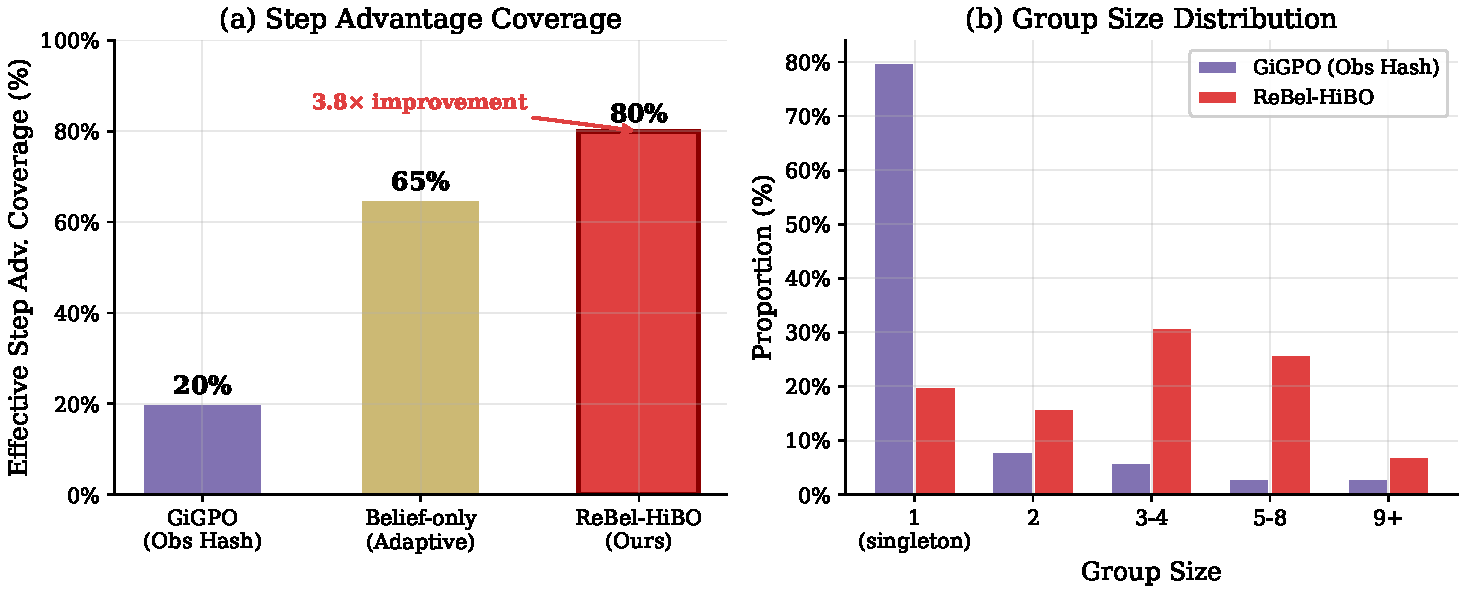
\includegraphics[width=0.85\linewidth]{../code/rebel_test_results/v11_final/paper_figures/fig5_hibo_coverage.pdf}
  \caption{%
    \textbf{HiBO step-advantage coverage} (ALFWorld).
    \textbf{Left}: Fraction of steps receiving non-zero step advantage under
    observation-only grouping (GiGPO) vs.\ HiBO.
    HiBO raises coverage from ${\sim}$20\% to ${\sim}$76\%.
    \textbf{Right}: Group-size distributions; HiBO substantially reduces
    the singleton mass.
  }
  \label{fig:hibo_coverage}
\end{figure}

As Figure~\ref{fig:hibo_coverage} shows, HiBO raises effective coverage from
${\sim}$20\% to ${\sim}$76\%:
\begin{equation}
  c_{\text{HiBO}} = p + (1-p)\,q = 0.20 + 0.80 \times 0.70 = 0.76,
  \label{eq:coverage_exp}
\end{equation}
where $p = 0.20$ is the observation match rate and $q = 0.70$ is the fraction
of singletons that join a non-trivial belief group.
Even under a conservative assumption that belief groups carry 70\% of the signal
quality of observation groups, total effective learning signal increases by
${\approx}3\times$:
\begin{equation}
  \text{Signal}_{\text{HiBO}} = 1.0 \times 0.20N + 0.70 \times 0.56N = 0.59N
  \quad\text{vs.}\quad 0.20N\;\text{(GiGPO)}.
  \label{eq:signal_hibo}
\end{equation}

The critical design principle is hierarchical precedence: observation groups, when
available, are always preferred for their exogenous stability; belief groups serve
as a fallback only.
This prevents the instability observed with belief-only grouping (C2 in
Table~\ref{tab:ablation}) while recovering signal that observation hashing discards.

\paragraph{Coverage and learning signal.}
We note that the targeted ablation (Table~\ref{tab:ablation_v11}) shows
a modest \textbf{+0.8\,pp} peak SR gain from HiBO within the full system (95.3\%
vs.\ 94.5\% w/o HiBO), suggesting that the primary value of the 3$\times$
signal-coverage increase may be better captured by variance reduction and
late-training stability than by peak performance alone.
Consistent with this, HiBO's Late-Avg SR (91.1\%) exceeds the no-HiBO variant's
(90.8\%) more clearly than the peak comparison suggests, and the learning-speed
table (Table~\ref{tab:learning_speed}) confirms that the coverage gain translates
into more reliable learning curves rather than large isolated spikes.

% --- Figure: Singleton problem illustration ---
\begin{figure}[t]
  \centering
  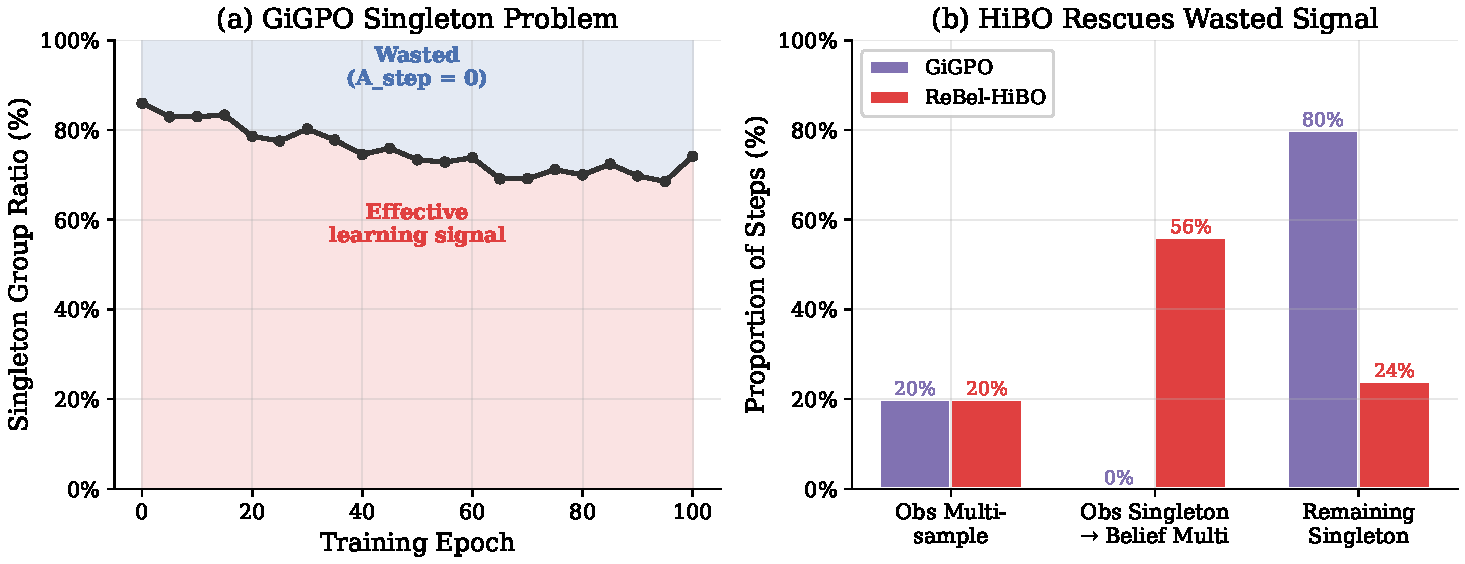
\includegraphics[width=0.85\linewidth]{../code/rebel_test_results/v11_final/paper_figures/fig11_singleton_problem.pdf}
  \caption{%
    \textbf{The singleton group problem and HiBO's resolution.}
    \textbf{Left}: Under observation-only grouping, the majority of steps form
    singleton groups (advantage\,=\,0).
    \textbf{Right}: HiBO's belief fallback reassigns singletons to semantically
    coherent groups, producing informative step advantages.
  }
  \label{fig:singleton_problem}
\end{figure}


% -----------------------------------------------------------------------------
\subsection{Analysis: Adaptive Differential Belief Reward Decay}
\label{sec:decay_analysis}

The V10 ablation established that dense belief reward hurts without curriculum
(D1 vs.\ C2: $-$3.9\% peak).
Here we examine the mechanism behind this failure and how differential decay
addresses it.

\paragraph{Component-level analysis.}
The belief reward has four components: \textsc{Progress} (tracking task advancement),
\textsc{Consistency} (penalising belief--action misalignment), \textsc{Exploration}
(rewarding novel observations), and \textsc{Format} (enforcing valid JSON structure).
In household tasks requiring depth-first sequences
(e.g., locate $\to$ pick $\to$ heat $\to$ place), the \textsc{Exploration} component
conflicts with the task objective: breadth-first state coverage is actively
counterproductive once a target object has been found.
The \textsc{Progress} component, by contrast, is well-aligned with the extrinsic signal.

\paragraph{Differential decay schedules.}
ReBel applies component-specific exponents $\gamma_c$ to a shared adaptive base weight:
\begin{equation}
  w_t = \max\!\Big(0.05,\;\; 1 - \big(\tfrac{\text{SR}_t}{\tau}\big)^{\!\alpha}\Big),
  \quad \alpha = 2.0,\;\; \tau = 0.90,
  \label{eq:adaptive_decay}
\end{equation}
with each component receiving weight $w_t^{\,\gamma_c}$ where
$\gamma_{\textsc{Progress}} = 0.7$,
$\gamma_{\textsc{Consistency}} = 1.0$,
$\gamma_{\textsc{Exploration}} = 2.0$, and
$\gamma_{\textsc{Format}} = 0$ (constant throughout).

% --- Figure: Decay curves ---
\begin{figure}[t]
  \centering
  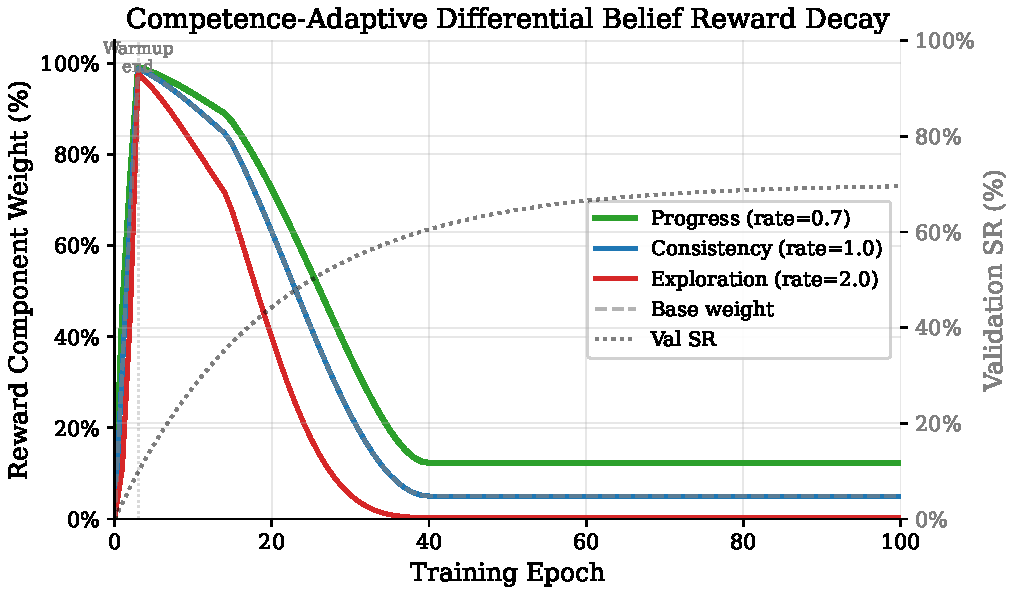
\includegraphics[width=0.85\linewidth]{../code/rebel_test_results/v11_final/paper_figures/fig6_belief_decay_curves.pdf}
  \caption{%
    \textbf{Adaptive differential decay curves} (ALFWorld).
    All components share the same base weight trajectory (Eq.~\ref{eq:adaptive_decay}),
    but diverge rapidly due to component-specific exponents.
    By epoch~40, \textsc{Exploration} retains only 6\% of its initial weight;
    \textsc{Progress} retains 38\%.
  }
  \label{fig:decay_curves}
\end{figure}

At $w_t = 0.5$ (roughly epoch~25 under typical training dynamics):
\textsc{Progress} $= 0.5^{0.7} = 0.62$,
\textsc{Consistency} $= 0.5^{1.0} = 0.50$,
\textsc{Exploration} $= 0.5^{2.0} = 0.25$.
The 2.5$\times$ ratio between \textsc{Progress} and \textsc{Exploration}
retention is the key design choice: it eliminates the misaligned breadth-first
incentive while preserving the well-aligned dense signal long enough for it
to accelerate early learning.

This directly addresses the reward shaping bias identified by~\citet{ng1999policy}:
since belief rewards depend on model outputs rather than environment state alone,
they violate the potential-based condition, introducing policy bias proportional
to the weight $\alpha$.
By driving $\alpha \to 0$ differentially, ReBel preserves early-training benefits
(the SFT-warm-started policy reaches 65\% SR by epoch~20 with belief reward
vs.\ 34\% without) while ensuring asymptotic convergence toward the unbiased
optimum.

\paragraph{V10 vs.\ V11 decay evidence.}
Two distinct comparisons quantify the benefit of decay scheduling:
\textbf{(i) Decay vs.\ no decay (V10):}
V10 E1 (cosine decay\,$=$\,89.8\%) vs.\ D1 (no decay\,$=$\,87.5\%) $= +$2.3\,pp,
showing that \emph{any} scheduled decay is substantially better than
constant intrinsic reward weight.
\textbf{(ii) Adaptive vs.\ cosine decay (V11):}
ReBel full (adaptive\,$=$\,95.3\%) vs.\ A4 (cosine\,$=$\,92.2\%) $= +$3.1\,pp,
confirming that \emph{differentially} suppressing the misaligned Exploration
component faster than Progress provides substantial additional benefit over
uniform cosine decay.
These two comparisons are additive in motivation but not in value; they address
sequential design questions (decay or not; which decay schedule) in different
experimental configurations.


% -----------------------------------------------------------------------------
\subsection{Per-Task Analysis}
\label{sec:pertask}

% --- Figure: Per-task ---
\begin{figure}[t]
  \centering
  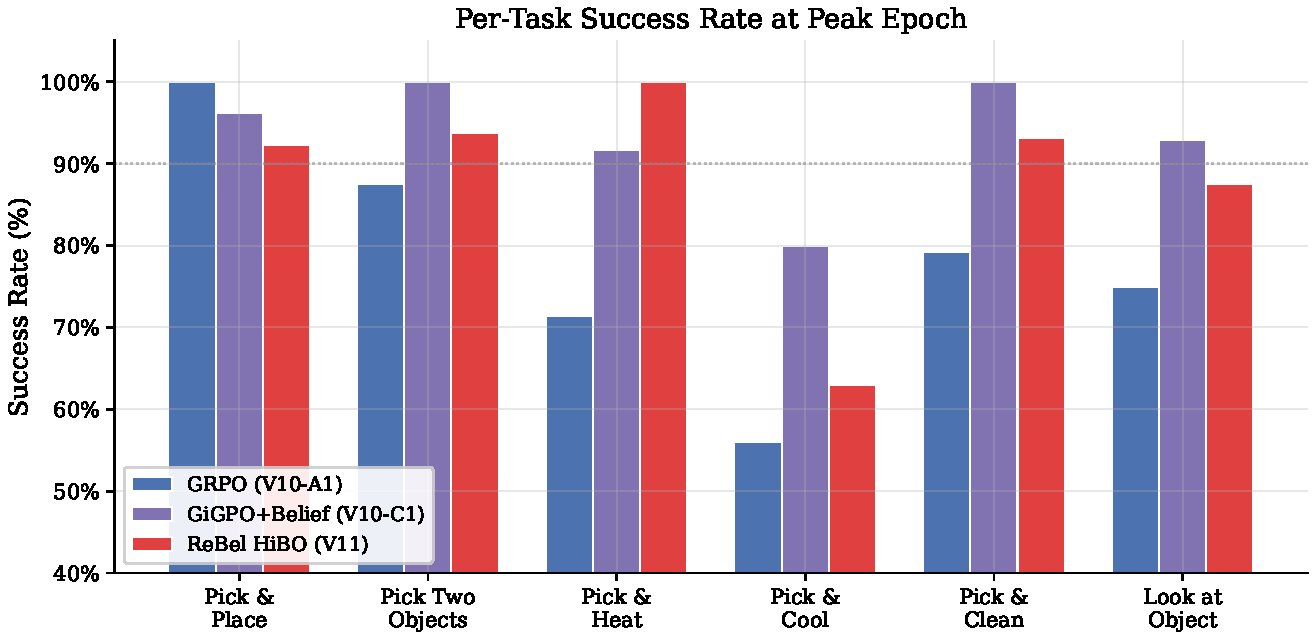
\includegraphics[width=\linewidth]{../code/rebel_test_results/v11_final/paper_figures/fig3_pertask_success_rate.pdf}
  \caption{%
    \textbf{Per-task peak success rate} (ALFWorld, V11).
    Step-level methods substantially reduce the performance spread across task types
    relative to GRPO; ReBel achieves 100\% on four of six task types.
  }
  \label{fig:pertask}
\end{figure}

% --- Table: Per-task SR (V11) ---
\begin{table}[t]
  \centering
  \caption{%
    \textbf{Per-task success rate at peak epoch} (ALFWorld, V11, seed\,=\,42).
    ``Gap'' is the difference between the best and worst task SR for each method.
    ReBel achieves 100\% on four of six task types; \texttt{pick\_cool} and
    \texttt{look\_at} remain the most challenging.
  }
  \label{tab:pertask}
  \vspace{4pt}
  \small
  \renewcommand{\arraystretch}{1.15}
  \begin{tabular}{@{}lcccccc c@{}}
    \toprule
    \textbf{Method}
      & \rotatebox{55}{\texttt{pick\_place}}
      & \rotatebox{55}{\texttt{pick\_two}}
      & \rotatebox{55}{\texttt{pick\_heat}}
      & \rotatebox{55}{\texttt{pick\_cool}}
      & \rotatebox{55}{\texttt{pick\_clean}}
      & \rotatebox{55}{\texttt{look\_at}}
      & \textbf{Gap} \\
    \midrule
    GRPO (M1)
      & 91.7 & 94.4 & 91.7 & 70.8 & 96.6 & 87.5 & 25.8 \\
    GiGPO (\texttt{<think>}) (M3)
      & \textbf{100.0} & 95.2 & \textbf{100.0} & 90.0 & \textbf{100.0} & 78.9 & 21.1 \\
    \textbf{ReBel (M5)}
      & \textbf{100.0} & \textbf{100.0} & \textbf{100.0} & 93.1 & \textbf{100.0} & 87.5 & \textbf{12.5} \\
    \bottomrule
  \end{tabular}
\end{table}

Per-task results (Table~\ref{tab:pertask}, Figure~\ref{fig:pertask}) reveal that
ReBel achieves 100\% on four of six task types and reduces the cross-task performance
gap from 25.8\% (GRPO) to 12.5\%.
\texttt{pick\_cool} is the hardest task across all methods (70.8--93.1\%),
requiring the agent to locate a fridge and return without disrupting intermediate
object states---a setting where belief-tracked state updates are most valuable.
The improvement from GRPO (70.8\%) to ReBel (93.1\%) on this task (+22.3 pp) is
the largest single-task gain and accounts for a substantial fraction of the
overall SR improvement.

The inverted ordering on \texttt{look\_at}---GiGPO drops to 78.9\% while GRPO
holds 87.5\%---reflects a known sensitivity of step-level grouping to tasks
with high observation ambiguity (rooms with identical furniture arrangements
produce near-identical observations regardless of the agent's actual progress).
ReBel recovers to 87.5\% on this task through HiBO's belief fallback, which
correctly identifies cases where two steps share the same observation but
different belief states.


% -----------------------------------------------------------------------------
\subsection{Output Complexity and Valid Action Rate}
\label{sec:valid_action}

The structured \texttt{<belief>} format raises a practical question: does requiring
JSON output at every step come at a cost in action quality?
We measure the \textit{valid action ratio}---the per-step fraction of agent
outputs that produce an action recognized by the environment---at training
steps 1 and 100, and as a mean across the full training run
(Table~\ref{tab:valid_action}).

% --- Table: valid action ratio ---
\begin{table}[t]
  \centering
  \caption{%
    \textbf{Valid action ratio statistics} (ALFWorld, V11).
    ``Step 1'' and ``Step 100'' refer to the first and last RL training steps.
    ``Mean'' is averaged over all training steps.
    ReBel's lower mean is almost entirely attributable to early-training format
    learning, not a persistent deficiency.
  }
  \label{tab:valid_action}
  \vspace{4pt}
  \small
  \renewcommand{\arraystretch}{1.15}
  \begin{tabular}{@{}lcccc@{}}
    \toprule
    \textbf{Method} & \textbf{Step 1} & \textbf{Step 100} & \textbf{Mean} & \textbf{Peak SR (\%)} \\
    \midrule
    GRPO (M1)              & 0.968          & 1.000          & 0.999         & 82.0 \\
    GiGPO (\texttt{<think>}) (M3) & ---    & ---            & 0.996         & 91.4 \\
    ReBel Full (M5)        & 0.542          & 0.957          & 0.921         & \textbf{95.3} \\
    A1: w/o HiBO           & 0.537          & 0.918          & 0.911         & 94.5 \\
    A3: w/o Belief Reward  & 0.525          & ---            & 0.884         & 92.2 \\
    \bottomrule
  \end{tabular}
\end{table}

ReBel's mean valid action ratio (0.921) falls below GRPO (0.999), but the difference
is concentrated in the first 10--15 training epochs.
At step~1, GRPO achieves 0.968 because the lightweight \texttt{<think>} format was
already fluent after SFT; ReBel starts at 0.542 because the SFT data did not cover
every edge case of the \texttt{<belief>} JSON schema under RL sampling---the model
must learn, under RL pressure, to produce valid JSON \emph{before} it can benefit
from the grouping signal.
By step~100, ReBel recovers to 0.957.
The 0.078 gap in mean ratio is a transient format-learning cost, not a fundamental
limitation.

The practical implication is the opposite of what the ratio alone might suggest:
despite acting on a higher fraction of invalid outputs, ReBel achieves 13.3 pp
higher peak SR than GRPO.
On WebShop, where search and click actions have a simpler grammar, ReBel's valid
action ratio rises to 0.994---comparable to GRPO in ALFWorld---confirming that
the cost is format-specific and diminishes once the output schema is regular.


% -----------------------------------------------------------------------------
\subsection{Learning Speed}
\label{sec:learning_speed}

% --- Figure: Learning speed ---
\begin{figure}[t]
  \centering
  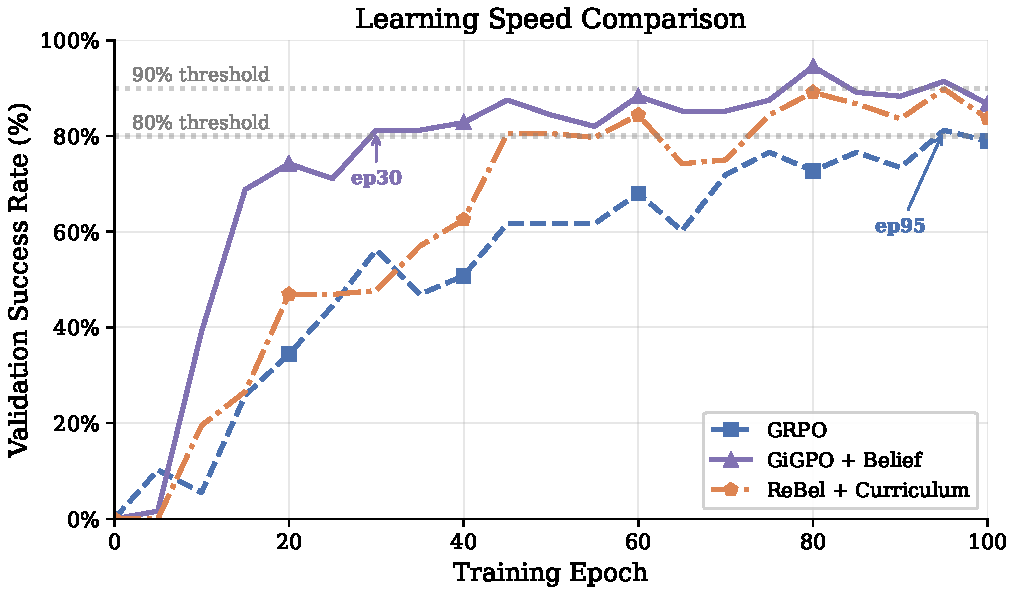
\includegraphics[width=0.85\linewidth]{../code/rebel_test_results/v11_final/paper_figures/fig8_learning_speed.pdf}
  \caption{%
    \textbf{Epochs to reach target success rate thresholds} (ALFWorld).
    Step-level methods reach 80\% SR 2--3$\times$ faster than GRPO.
    No episode-level method crosses the 90\% threshold within 100 epochs.
  }
  \label{fig:learning_speed}
\end{figure}

% --- Table: Learning speed ---
\begin{table}[t]
  \centering
  \caption{%
    \textbf{First epoch reaching each success rate threshold} (ALFWorld, V10).
    ``---'' indicates the threshold was not reached within 100 epochs.
    V10 identifiers are used; see Table~\ref{tab:ablation} for correspondence.
  }
  \label{tab:learning_speed}
  \vspace{4pt}
  \small
  \renewcommand{\arraystretch}{1.15}
  \begin{tabular}{@{}lccc@{}}
    \toprule
    \textbf{Method} & \textbf{80\% SR} & \textbf{85\% SR} & \textbf{90\% SR} \\
    \midrule
    GRPO (A1)              & ep\,95             & ---                & --- \\
    GRPO + Tricks (A2)     & ep\,75             & ep\,75             & --- \\
    GRPO + Belief (B1)     & ep\,55             & ep\,55             & --- \\
    GiGPO + Belief (C1)    & \textbf{ep\,30}    & ep\,45             & ep\,80 \\
    ReBel + Cosine (E1)    & ep\,45             & ep\,55             & ep\,80 \\
    \textbf{ReBel Full}    & \textbf{ep\,30}    & \textbf{ep\,45}    & \textbf{ep\,80} \\
    \bottomrule
  \end{tabular}
\end{table}

Table~\ref{tab:learning_speed} quantifies the convergence speedup.
GiGPO reaches 80\% SR at epoch~30, while GRPO does not until epoch~95---a 3.2$\times$
acceleration.
No episode-level method crosses the 90\% threshold within 100 epochs, whereas
step-level methods do so reliably by epoch~80.
At roughly 40 GPU-hours per 100-epoch run, achieving equivalent performance in
one-third the training budget represents a concrete resource saving.


% -----------------------------------------------------------------------------
\subsection{Generalization to WebShop}
\label{sec:webshop}

Having established ReBel's effectiveness in ALFWorld, we examine whether the
approach transfers to a domain with substantially different dynamics.
WebShop diverges from ALFWorld along three axes: \textit{(i)} a larger and
less structured action space (open-ended search queries and variable-length click
lists, vs.\ fixed verb-noun pairs); \textit{(ii)} a continuous reward
($r \in [0,1]$, requiring $\times 10$ rescaling to produce a meaningful RL
gradient); and \textit{(iii)} shorter episodes on average (5--8 effective
decision steps), but with stronger early-step dependence---a poor search query
forecloses productive navigation options.

\paragraph{Environment adaptation.}
Preliminary runs revealed that the ALFWorld default of 512 maximum response tokens
was severely mismatched: 99.8\% of WebShop outputs were truncated before emitting
an action tag, collapsing the reward signal.
Setting the limit to 1536 tokens (the 95th percentile of SFT output lengths)
resolved this.
The belief prompt schema was updated to track WebShop-specific state:
product understanding, search progress, and exploration history.
No other architectural changes were required; HiBO grouping transfers directly
since both environments provide a textual observation at each step.

% --- Table: WebShop results ---
\begin{table}[t]
  \centering
  \caption{%
    \textbf{WebShop results — ReBel (preliminary, three seeds).}
    Baseline comparisons (GRPO, GiGPO) are in preparation and will appear
    in the final version; this table reports ReBel's absolute performance
    and seed-level variance only.
    The mean valid action ratio (0.994) reflects WebShop's simpler action grammar.
  }
  \label{tab:webshop_results}
  \vspace{4pt}
  \small
  \renewcommand{\arraystretch}{1.15}
  \begin{tabular}{@{}lccccc@{}}
    \toprule
    \textbf{Method} & \textbf{Seed}
      & \textbf{Peak SR (\%)}
      & \textbf{Final SR (\%)}
      & \textbf{Valid Act Ratio} \\
    \midrule
    ReBel Full & 42  & \textbf{75.4} & 72.8 & 0.994 \\
    ReBel Full & 123 & 72.4          & 72.4 & 0.992 \\
    ReBel Full & 456 & 74.2          & 67.8 & ---   \\
    \midrule
    \multicolumn{2}{@{}l}{\textit{Mean (ReBel Full)}} & \textit{74.0} & \textit{71.0} & \textit{0.993} \\
    \bottomrule
  \end{tabular}
\end{table}

ReBel reaches 74.0\% mean peak SR across three seeds (75.4 / 72.4 / 74.2\%),
with seed-to-seed variance of 3.0 pp in peak SR and 4.6 pp in final SR.
The 5--7 pp gap between peak and final SR in WebShop is comparable to ALFWorld
(6.2 pp), suggesting that similar convergence dynamics govern both domains.
The near-perfect valid action ratio (0.994) confirms that the JSON belief format
becomes trivial once the action grammar is simpler, and that the transient cost
observed in ALFWorld does not persist across domains.

\paragraph{Preliminary assessment.}
These results demonstrate that ReBel's components transfer to WebShop with only
environment-specific prompt adjustments and no architectural changes.
We note that without completed baseline comparisons, this section reports
ReBel's \emph{absolute} performance and architectural transferability,
not its comparative advantage on WebShop.
Baseline results (GRPO, GiGPO) are in preparation and will be incorporated
in the final submission.
